The design of a web interface for an automated robotic workcell must prioritize user experience, system performance, and availability. In this section, we delve into the key components of a web-based UI that allows operators to monitor and control the system effectively, ensuring streamlined performance during sheet metal bending process. The web interface uses the React.js framework for the front end and integrates with ROS (Robot Operating System) for robot control and 3D visualization of workcell. React.js is a component based development environment. This means even if a single component on the screen fails, the interface wouldn't crash. The web interface is currently hosted locally on port 3000. It is possible to make this web interface available on the internet, but that would require hosting on a 24/7 available server and a domain.


The web interface has two main sections, viewer and ROS control panel. Viewer is used for visualizing and monitoring the KR1410 robot in the workcell. The second section include buttons and sliders which controls the robot loaded in the viewer.

\begin{figure}[h]
    \centering
    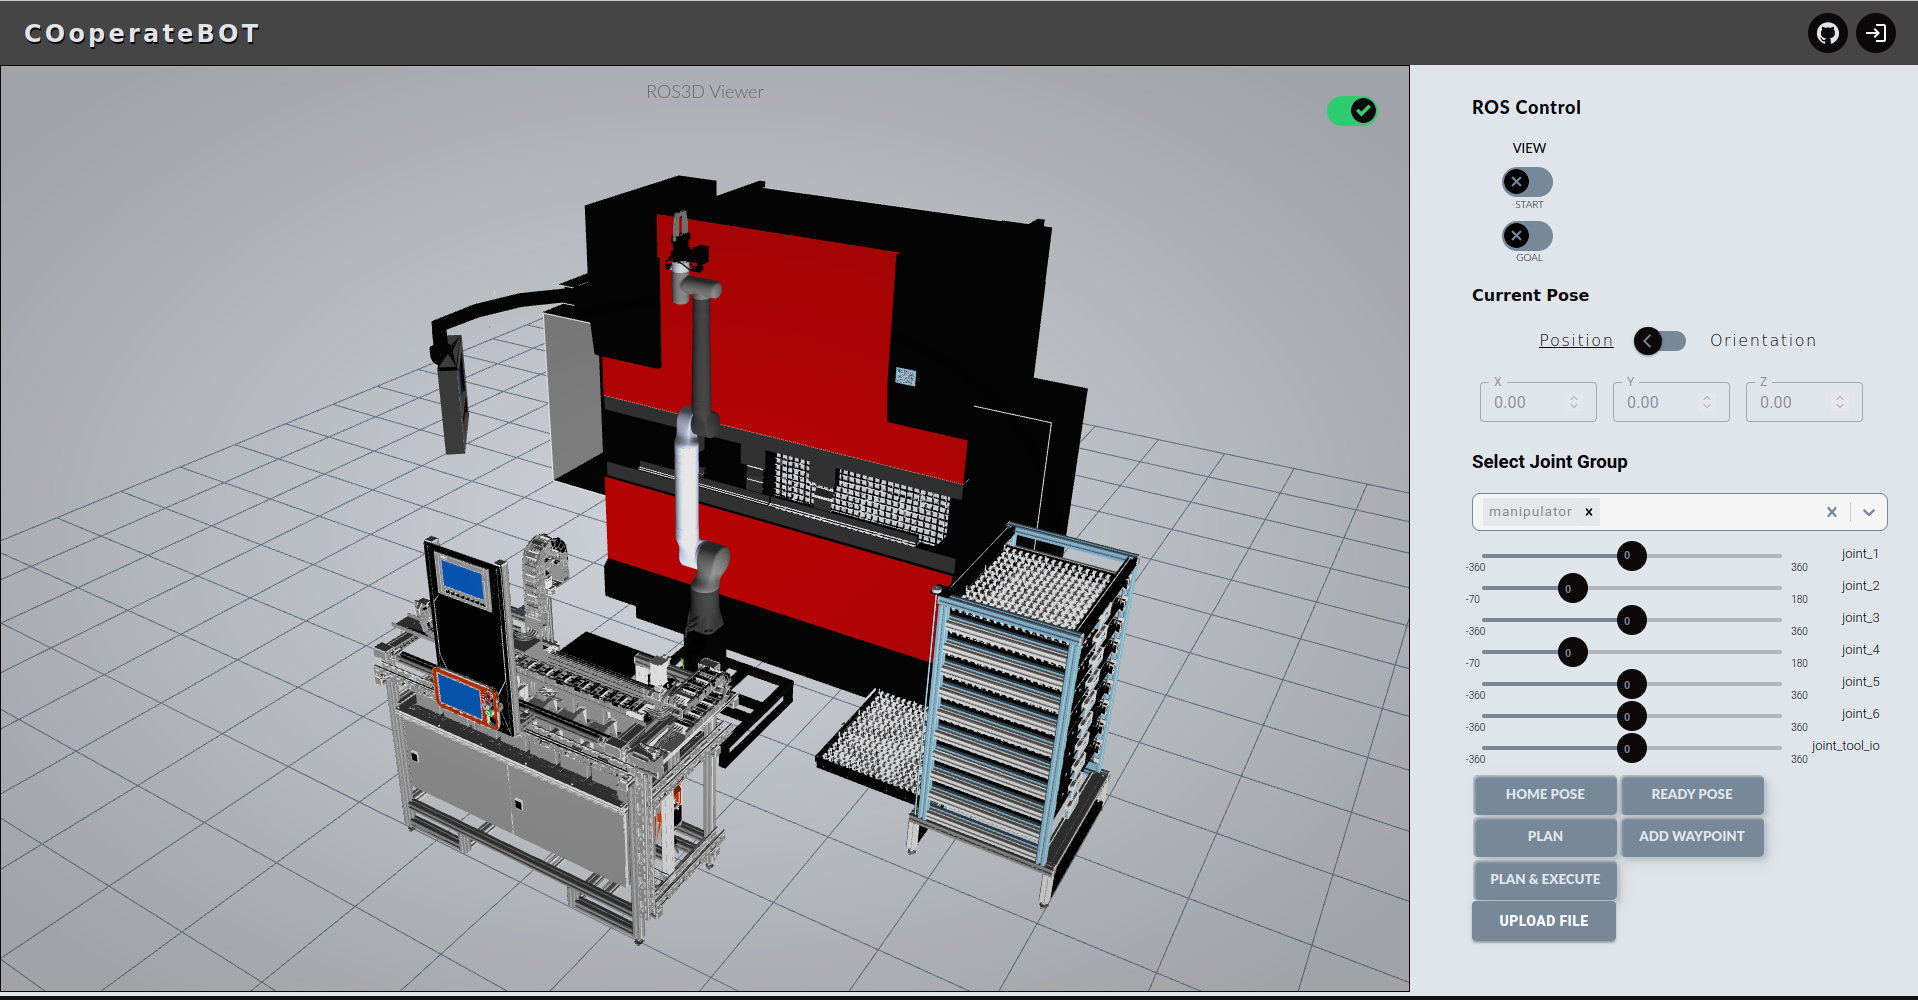
\includegraphics[width=1\textwidth]{figures/webui/webui0.png}
    \caption{Web User Interface}
    \label{fig:web-ui}
\end{figure}

\subsection{Viewer}
\label{subsec:web-ui-viewer}
The Viewer component provides a 3D visualization of the robot model within the web application. It leverages ros3djs to render a real-time representation of the robot, including its physical structure and the workspace. Users can manipulate the camera to explore the robot from various angles, zoom in and out, and observe its movements in real-time as it receives ROS data.

The viewer is customizable, with options to control the size, background color, change workspace models, and field of view to optimize visualization based on user needs. This is particularly useful for monitoring the robot's operations in complex environments. However, this would require a web server restart.

The viewer has two modes: simulation mode and reality mode. It has a button on the top right side, which allows switching from gazebo simulations to real robot. Hence allowing simulations or controlling of real robot directly from a single interface without the need to restart the web server. This prevents errors in real-world operations and ensures that the robot performs the necessary movements accurately and collision-free after testing in simulations.


\subsubsection{Auto connection}
\label{subsubsec:web-ui-auto-connection}
To ensure smooth operations, the Auto connection feature establishes a real-time link between the robot and the web interface via WebSocket, utilizing the Rosbridge package. This connection facilitates the exchange of sensor data, system state information, and control commands, allowing for immediate responses.

The Auto Connection feature is build on \textbf{AutoRos} package which can handle intermittent network failures by automatically re-establishing the WebSocket connection when needed. This reduces downtime and ensures that the system remains responsive, even in situations where network instability might otherwise interrupt operations.

\subsubsection{Robot URDF Visualization}
\label{subsubsec:web-ui-urdf-visualization}
The Unified Robot Description Format (URDF) visualization provides a detailed, kinemtic model of the robot within the web interface. This feature uses ROS to generate a real-time model of the robot using ROS parameter \textit{robot\_description}, showcasing its joints, links, and kinematics. The URDF model is not just a static image; it actively updates as the robot moves using ROS topic \textit{$\backslash$joint\_states}, providing valuable informtion about the robot's physical status and positioning in the workcell.

There are three Robot URDF visualizations in the web UI as illustrated in figure \ref{fig:web-ui-preview}. The green marked robot is for determining the starting pose of the robot from which path planning begins. The red URDF model of robot is the target pose to perform path planning to. The grey robot URDF models shows the current pose of the robot either in Gazebo simulator or real world.

\subsubsection{Interactive Marker}
\label{subsubsec:web-ui-interactive-marker}
Interactive markers enable direct manipulation of the robot's joint in the web interface. Using a drag-and-drop interface, operator can position the robot's TCP in the desired position and automatically change the robot configuration. This is particularly useful for tasks such as path planning between stations or small adjustments in the robot's pose.

By interacting with the interative marker in the Viewer, operator can simulate robot movements before sending final commands. The interactive marker is controlled and updated with the MoveIt package, which performs motion planning and collision avoidance in the background.


\subsection{ROS Control Panel}
\label{subsec:web-ui-ros-control}
The ROS Control panel is on the right side of the web interface. It includes several inputs and buttons through which operator can interact with the robot in the viewer. Designed with usability and accessibility in mind, the control panel offers various functionalities for real-time robot operation, task management, and motion planning. The control panel is divided into several key sections, which includes manipulating start/target URDF models, showing current TCP pose, joint configuration and other control buttons. The key subcomponents of the ROS Control Panel are elaborated below.



\begin{figure}[h]
    \centering
    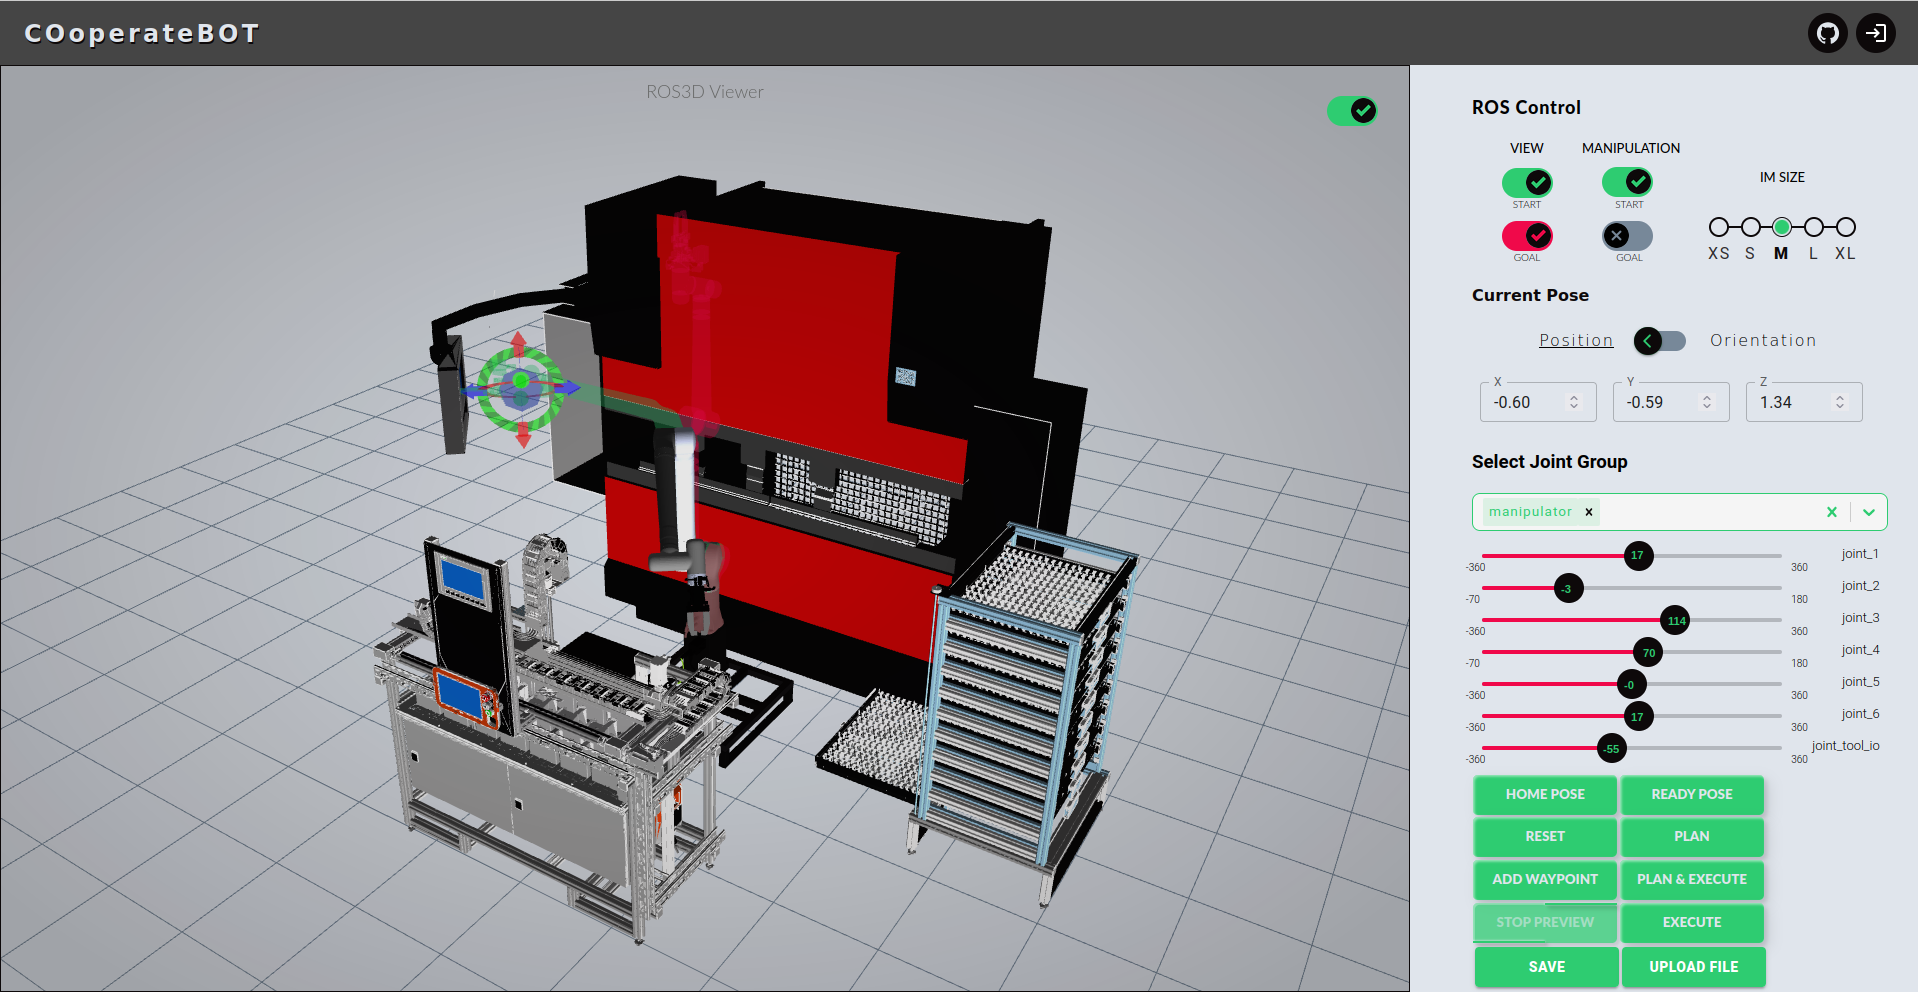
\includegraphics[width=1\textwidth]{figures/webui/web-ui-preview.png}
    \caption{Web User Interface previewing task execution}
    \label{fig:web-ui-preview}
\end{figure}

\subsubsection{View and Manipulation}
\label{subsubsec:web-ui-view-manipulation}
Motion is always planned from the start robot URDF model (green) to target robot URDF model (red). Unless the reality mode is turned on which plans from the current pose of the robot (grey) to the target robot URDF model (red). \textbf{View} toggle switch shows the start/target robot model respectively. \textbf{Manipulation} toggle allows the manipulation of the start/target robot model in the viewer. Only one Robot model in the viewer can be actively manipulated at a time.


\subsubsection{Interactive marker size}
\label{subsubsec:web-ui-im-size}
This settings changes the size of interactive marker on the start/target robot model. It helps in the precise placement of the TCP in the robot workcell. A smaller interactive marker would be able to make small movements during zoom-in. In total, there are five sizes of interactive markers available in the web interface.


\subsubsection{Current pose}
\label{subsubsec:web-ui-current-pose}
The \textbf{Current pose} section always shows the TCP pose of the real robot (or simulated robot from gazebo) from the viewer. The TCP pose has three position coordinates (X,Y,Z) and euler angles (R,P,Y).

\subsubsection{Joint Slider}
\label{subsubsec:web-ui-joint-slider}
The joint shows the joint configuration of active URDF robot model. If both the \textbf{Manipulation} toggle switch are in off position, the joint configuration of the real robot or gazebo simulator robot is shown. The joint configuration can be changed by sliding the slider for the respective joint.

\subsubsection{Buttons}
\label{subsubsec:web-ui-buttons}
The control panel has several buttons for controlling the robotic arm. There are two main buttons which always allows the robot to come back to home position or ready position from any joint configuration. These are \textbf{HOME POSE} button and \textbf{READY POSE} button respectively. \textbf{RESET} button allows resetting the start and target robot model in the viewer to current robot joint configuration.

\textbf{PLAN} allows trajectory planning from start robot model to target robot model. If the planning is successful, few other buttons will show up like \textbf{PREVIEW} and \textbf{EXECUTE}. \textbf{PREVIEW} shows how the robot will move on the planned trajectory path without actually moving the real robot. 

\textbf{EXECUTE} allows the planned path to be executed on the real robot. It is necessary in this case that start robot model matches the configuration of current robot model.

\textbf{ADD WAYPOINT} button also does path planning, but allows adding a new pose in the world by moving the target robot model. This allows adding multiple waypoints to a target pose without actually overwriting a previously planned path.

\textbf{PLAN \& EXECUTE} allows both path planning and then execution of path from current robot model to the target pose.

\vspace{\baselineskip}
The web interface includes options for saving and loading pre-planned paths. \textbf{SAVE} buttons allows saving the planned path in a \textit{.json} file. 
These stored paths are essential for repeatable bending operations such as bending metal sheets of the same dimensions. By saving a successful bending operation's trajectory, operators can easily load it for future tasks, reducing downtime of robot and ensuring consistent results. This saved file can be loaded back in the interface using the \textbf{UPLOAD FILE} button. This feature allows testing and handling multiple workpiece variants by providing quick access to previously tested paths. The ability to save and load paths makes the workcell more flexible and adaptable, as operators can switch between tasks without needing to reprogram the robot from scratch.


